\chapter{Volba vhodné technologie}
Pro tuto síť nejsou v tuto chvíli stanoveny zadávající firmou žádné konkrétní požadavky na hardware. Proto je možné vybrat z hlediska softwarového řešení jakoukoliv platformu. Z hardwarového hlediska je doporučeno používat evaluační desky od STMicroelectronics. V následující části budu popisovat jednotlivé použité technologie a důvod jejich volby.

\section{Prvky senzorické sítě}
Prvky senzorické sítě jsou testovány na vývojových deskách s mikrokontroléry STM32F207IGH6 a STM32F457IGH6 s využitím oficiálních Cube knihoven \cite{cube}. Jedná se o 32-bit mikrokontroléry pro obecné použití. Pro oba mikrokontroléry dále platí, že mají 176 pinů s velikostí flash paměti 1024 KB v provedení pouzdra UFBGA pro běžné rozsahy teplot od -40 do 85 °C.

\begin{figure}[h]
    \centering
	\makebox[\textwidth]{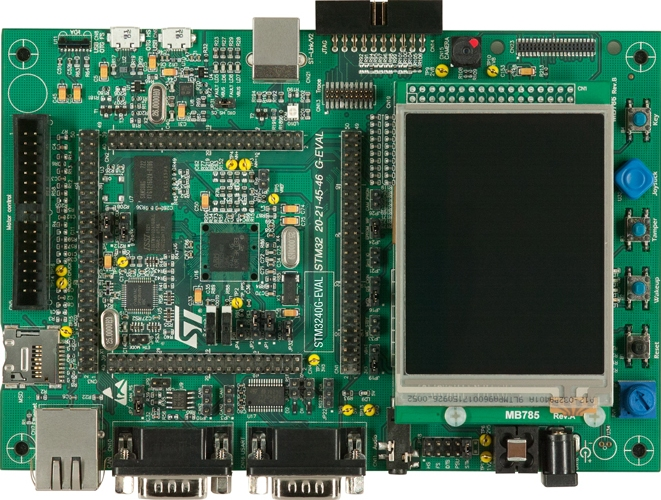
\includegraphics[width=\textwidth]{img/eval_board.jpg}}
	\caption{Použitá vývojová deska} %TODO dopsat typ (označení) desky
	\label{fig:eval-board}
\end{figure}

\subsection{Procesor STM32F207IGH6}
\begin{itemize}
\itemsep0em
\item Jádro ARM 32-bit Cortex\texttrademark-M3 CPU (120 MHz max)
\item 128 KB SRAM
\item LCD interface
\item 12 \ensuremath{\times} 16-bit timer, 2 \ensuremath{\times} 32-bit timer - až 120 MHz
\item 15 komunikačních rozhraní
\item 2 \ensuremath{\times} USB, 10/100 Ethernet
\item 8 až 14-bit interface pro kameru
\item CRC jednotka
\end{itemize}

\subsection{Procesor STM32F457IGH6}
\begin{itemize}
\itemsep0em
\item Jádro ARM 32-bit Cortex\texttrademark-M4 CPU (168 MHz max)
\item 192 KB SRAM
\item LCD interface
\item 12 \ensuremath{\times} 16-bit timer, 2 \ensuremath{\times} 32-bit timer - až 168 MHz
\item 15 komunikačních rozhraní
\item 2 \ensuremath{\times} USB, 10/100 Ethernet
\item 8 až 14-bit interface pro kameru
\item CRC jednotka
\end{itemize}

Veškeré vývojové desky s mikrokontroléry jsou připojeny pomocí klasických síťových prvků a UTP kabelů do serveru.

\section{Real-time server}
Jako real-time server, který obsluhuje celou síť i webovou aplikaci je zvolen Node.js \cite{nodejs}. Jedná se o platfomu postavenou nad V8 JavaScript Engine od společnosti Google. V8 je engine napsaný v C++, který využívá například prohlížeč Google Chrome jako jádro pro velmi rychlé zpracování javascriptu. Díky tomu je možné využívat téměř všech vlastností javascriptu, zejména pak single-thread asynchronní chování (non-blocking I/O model) a EDA architektury. Jedná se o velmi podobný engine jako je v prohlížeči Google Chrome s tím rozdílem, že Node.js neobsahuje možnost práce s oknem programu, nebo s dokumentem jako takovým, protože zde žádný není. Oproti tomu umožňuje přistupovat k process objektu, který zase není dostupný v prohlížečích. Následující ukázka ukazuje jednoduchý webový server napsaný právě s pomocí Node.js:

\begin{minted}[linenos,breaklines]{javascript}
var http = require('http');
var PORT = 8000;

var server = http.createServer(function(request, response) {
	response.writeHead(200, {'content-type': 'text/html'});
	response.write("<h1>hello</h1>\n");
	setTimeout(function() {
		response.end("<p>world</p>\n");
	}, 2000);
});

server.listen(PORT, function() {
	console.log('Server is listening on port ' + PORT);
});
\end{minted}

Tento server je zároveň vysoce škálovatelný a to hlavně do šíře. Je tak možné vytvořit velký počet vzájemně komunikujících uzlů (node), které spolu komunikují. Tyto uzly jsou však striktně odděleny (i na úrovni paměti) a nemohou se tak přímo ovlivňovat. Tento model je vhodný pro velmi vytížené aplikace, protože je možné potřebný výkon rozložit na velké množství méně výkonných strojů.

\section{Databázový server}
Na pozici databázového serveru byl zvolen Redis \cite{redis}. Redis je key-value databáze. Od nejrozšířenějších relačních databázích se liší například tím, že je násobně výkonnější a neobsahuje relace. Významným prvkem této databáze je právě vztah klíče a hodnoty, kdy hodnotu je možné ukládat do sedmi datových struktur (string, hash, list, set, sorted set, bitmap, hyperloglog). Velkou rychlost Redisu zajišťuje zejména to, že pracuje s RAM pamětí serveru. Přijaté hodnoty si nejdříve ukládá právě do paměti a následně je podle konfigurace ukládá na disk. Příklad výchozí konfigurace:

\begin{minted}[breaklines]{text}
# save <seconds> <changes>
save 900 1
save 300 10
save 60 10000
\end{minted}

Vždy musí být splněna časová podmínka i množství změn za tento čas. Takové nastavení pak tedy udává, že se po 900 vteřinách (15 minut) uloží změny na disk, pokud byla provedena změna alespoň jednoho klíče, nebo po 300 vteřinách při změně alespoň deseti klíčů, resp. po minutě, došlo-li ke změně alespoň 10 000 klíčů. Již z této konfigurace je zřejmé, že se u Redisu očekává velké vytížení a tato databáze je na to připravena.

\subsection{Redis klíče}
%TODO počeštit binary safe
Redis klíče mohou být velké až 512 MB a jsou binary safe, tzn. že platný je jak běžný text, tak prázdný text, ale také binární data, nebo obsahy souborů (do maximální velikosti klíče). Samotným klíčům lze pak také nastavovat životnost (pomocí příkazu \texttt{EXPIRE}). Klíče potom vyprší po nastaveném čase.

\subsection{Datová struktura string}
Datová struktura string je nejzákladnější způsob jak je možné uložit data do databáze. Princip je velmi jednoduchý. Každému klíči se přiřadí textová hodnota. V této práci je datová struktura string používána k ukládání a inkrementování celkového počtu přijatých nebo odeslaných zpráv. Ukázka použití počítadla:

\begin{minted}[breaklines]{text}
> SET counter 1
OK
> INCR counter
(integer) 2
> INCRBY counter 50
(integer) 102
> INCRBYFLOAT counter 3.0e3
"3102"
\end{minted}

Časová náročnost těchto operací je O(1)\footnote{Označení $O(f(x))$ značí asymptotickou složitost algoritmu. Složitosti algoritmů rozdělujeme do různých tříd ($1 < log(n) < n < n\cdot log(n) < n^k < k^n < k! < n^n$), které určují jak je daný algoritmus rychlý. Zápisy je pak možné číst tak, že algoritmus je stejně rychlý, nebo rychlejší, než $f(x)$.}.

\subsection{Datová struktura hash}
Hash je velmi podobný stringu s tím rozdílem, že je možné ukládat k jednomu klíči více hodnot. Časová složitost je pak O(1) pro jeden prvek resp. O(N) kde N je počet ukládaných nebo vybíraných prvků. V této práci je datová struktura hash použita právě pro ukládání informací o koncovém zařízení. Konkrétně se o koncových zařízeních uchovává IP adresa, porty TCP a UDP komunikace, čas posledního ohlášení, status aktivity a počet přenesených zpráv.

\subsection{Datová struktura list}
List je v Redisu implementovaný jako spojový seznam. Tato implementace umožňuje vkládat nová data na začátek, nebo na konec spojového seznamu v konstantním čase nezávisle na počtu prvků v seznamu. Časová složitost je tedy opět O(1). U operací kdy se vkládá prvek dovnitř seznamu je složitost O(N), kdy N je počet prvků, přes které je nutné iterovat, než se dostaneme k požadovanému umístění. V nejlepším případě muže být tedy i zde časová složitost O(1). List je v tomto projektu použitý pro ukládání historie příchozích dat z koncentrátorů následovně:

\begin{minted}[breaklines]{text}
> LPUSH device_uid:data <data>
> LTRIM device_uid:data 0 999
\end{minted}

Výhodné na tomto přístupu je to, že je složitost obou příkazů O(1). Je to dáno tím, že LPUSH umisťuje data do seznamu zleva což není nijak časově náročné a dále složitost LTRIM funkce je dána počtem prvků, které se touto funkcí odstraní, což je jeden starý. S minimální režií je tak uchováváno posledních 1000 hodnot.

\subsection{Datová struktura set a sorted set}
Sety jsou neseřazené kolekce unikátních stringů. Zde je nutné zdůraznit, že hodnoty zde skutečně nejsou seřazeny a vracený výsledek tak může měnit pořadí. Výhodné je, že je možné do této množiny ukládat data se složitostí O(N), kde N je počet prvků. To samé platí i pro čtení. Tato struktura se hodí pro ukládání relací čímž je možné simulovat relační vztahy mezi objekty. V tomto projektu je proto set používaný pro ukládání všech známých zařízení k síti a dále pro ukládání vazeb mezi jednotlivými koncentrátory.

Sorted set je obdoba setu s tím rozdílem, že prvky jsou v množině seřazeny podle zvoleného skóre. Tato struktura není v projektu nikde použita a je zde uvedena pouze pro úplnost.

\subsection{Datová struktura bitmap}
Bitmapy umožňují ukládat binární data do databáze. Tento způsob práce s daty je pouze obdobou práce se stringy. Vzhledem k tomu, že se jedná o práci s nejmenší jednotkou informace, je tato struktura velmi úsporná co se týče velikosti a velmi se hodí pro ukládání velkého množství pravdivých resp. nepravdivých informací. Bitmapy jsou limitovány na velikost 512 MB stejně jako klíče. To jinými slovy znamená, že je v jednom klíči možné uchovat informace až o $2^{32}$ stavech ($2^{32} = 4\,294\,967\,296\,b = 536\,870\,912\,B = 524\,288\,kB = 512\,MB$).

Tato struktura není v projektu nikde použita a je zde uvedena pouze pro úplnost.

\subsection{Datová struktura hyperloglog}
Posledním a relativně novým datovým typem je hyperloglog. Jedná se o statistickou datovou strukturu, která se používá zejména pro rychlé určení kvantity unikátních dat s chybou méně než 1\%. Tato struktura předchází paměťové náročnosti při počítání množství unikátních dat. V běžném případě je totiž nutné pamatovat si tyto data, aby bylo možné při dalším vstupu unikátní hodnotu započítat, nebo ji ignorovat, protože je již započítána. Redis při své implementaci používá konstantní množství paměti, konkrétně 12 kB v nejhorším případě.

Tato struktura není v projektu nikde použita a je zde uvedena pouze pro úplnost.

\subsection{Výkon Redisu}
Redis díky svému přístupu k paměti a omezenému počtu zapisování na disk je velmi rychlá databáze. Dále je připravena na škálování do šíře, takže je možné připojit další servery jako databázové uzly \cite{redis-cluster}. Níže je uvedený reálný výsledek benchmarku \cite{redis-benchmark} na Linuxovém stroji Debian s 2\texttimes CPU po 2 GHz, 2 GB RAM. Test je proveden pro různé datové struktury a jejich příkazy vždy pro 50 souběžných připojení a 100 000 požadavků s délkou SET/GET hodnoty 256 B. V tomto prvním testu jsou vždy příkazy posílány postupně a postupně také vybavovány.

\begin{minted}[linenos,breaklines]{text}
$ redis-benchmark -q -n 100000 -d 256
PING_INLINE: 212314.23 requests per second
PING_BULK: 211416.50 requests per second
SET: 131752.31 requests per second
GET: 199600.80 requests per second
INCR: 213219.61 requests per second
LPUSH: 213219.61 requests per second
LPOP: 204918.03 requests per second
SADD: 214592.28 requests per second
SPOP: 212765.95 requests per second
LPUSH (needed to benchmark LRANGE): 213675.22 requests per second
LRANGE_100 (first 100 elements): 45269.35 requests per second
LRANGE_300 (first 300 elements): 15586.04 requests per second
LRANGE_500 (first 450 elements): 9325.75 requests per second
LRANGE_600 (first 600 elements): 6472.49 requests per second
MSET (10 keys): 131578.95 requests per second
\end{minted}

Je zřejmé, že již při základní konfiguraci dosahuje Redis vysokých výkonů. Nevýhodou této konfigurace, resp. přístupu k práci s Redisem, je skutečnost, že nový požadavek je vždy poslán až po zpracování databází a vrácení odpovědi. Redis totiž funguje pomocí TCP, takže klient odesílá požadavek a přijímá od serveru odpověď. Tato smyčka může být velmi krátká, zejména pak pokud je redis umístěn na stejném serveru jako klient. V každém případě však vzniká časová prodleva mezi tím, kdy putují pakety od klienta k serveru a zpět. Tento čas se nazývá RTT a i čas potřebný pro lokální smyčku na serveru může být v součtu velký při velkém počtu požadavků. Tento problém se dá částečně vyřešit tzv. pipeliningem. Pak je možné posílat více zřetězených požadavků v jednom dotazu. Následující příklad ukazuje stejný benchmark jako dříve, ale se zapnutým pipeliningem. Vždy se zřetězí 16 příkazů do jednoho požadavku:

\begin{minted}[linenos,breaklines]{text}
$ redis-benchmark -q -n 100000 -d 256 -P 16
PING_INLINE: 1612903.25 requests per second
PING_BULK: 2127659.75 requests per second
SET: 1086956.50 requests per second
GET: 1351351.38 requests per second
INCR: 1219512.12 requests per second
LPUSH: 934579.44 requests per second
LPOP: 1030927.81 requests per second
SADD: 1265822.75 requests per second
SPOP: 1562499.88 requests per second
LPUSH (needed to benchmark LRANGE): 990099.00 requests per second
LRANGE_100 (first 100 elements): 35186.49 requests per second
LRANGE_300 (first 300 elements): 8521.52 requests per second
LRANGE_500 (first 450 elements): 5236.70 requests per second
LRANGE_600 (first 600 elements): 3888.48 requests per second
MSET (10 keys): 207468.88 requests per second
\end{minted}

%TODO REDIS - test dotazové smyčky pro delší segmentovou síť viz poznámky p. Krista

\subsection{RESP protokol}
Redis databáze komunikuje interně přes TCP v RESP (Redis Serialization Protocol) formátu. RESP používá celkem 5 typů dat. Vždy platí, že první byte je byte určující o jaký formát se jedná:

\begin{itemize}
\itemsep0em
\item \texttt{+} simple string (jednoduchý řetězec)
\item \texttt{-} error (chybový stav)
\item \texttt{:} integer (celé číslo)
\item \texttt{\$} bulk string (binary safe řetězec)
\item \texttt{*} array (pole)
\end{itemize}

Následuje samotný obsah, nebo dodatečné informace, například o délce a vše je ukončeno pomocí \texttt{CRLF} (\texttt{\textbackslash r\textbackslash n}). Postupně tedy přenášené informace mohou vypadat například takto:

\begin{itemize}
\itemsep0em
\item \texttt{+PONG\textbackslash r\textbackslash n}
\item \texttt{-Error 123\textbackslash r\textbackslash n}
\item \texttt{:54986\textbackslash r\textbackslash n}
\item \texttt{\$4\textbackslash r\textbackslash nPING\textbackslash r\textbackslash n} (první část určuje délku bulk stringu, NULL je pak \texttt{\$-1\textbackslash r\textbackslash n})
\item \texttt{*2\textbackslash r\textbackslash n\$3\textbackslash r\textbackslash nGET\textbackslash r\textbackslash n\$3\textbackslash r\textbackslash nkey\textbackslash r\textbackslash n} (první je délka pole, následuje kombinace předchozích)
\end{itemize}

Redis server potom přijímá podle řetězců obsahující jednotlivé instrukce. Tento protokol je velmi důležitý, protože i koncentrátory posílají data (přes TCP i UDP) v RESP formátu, je tak možné data posílat přímo do databáze. Tato vlastnost však není využívána, protože je vhodné, aby byl jako prostředník server a například zjišťoval aktivitu koncentrátorů. Každopádně tato možnost zde je a pokud by bylo zapotřebí ukládat data tou nejrychlejší cestou, přímý přístup do databáze je tímto možný a funkční.

\section{Webová aplikace}
Webový server je možné spustit na již běžícím Node.js serveru. Pro webovou aplikaci byl zvolen framework Sails.js \cite{sails}. Sails je MVC webový framework, který staví právě nad Node.js, ale ulehčuje práci při stavbě webových aplikací. Výhodou tohoto přístupu je to, že je možné na jednom serveru zapnout jak server zpracující požadavky z koncentrátorů, tak server obsluhující požadavky klientů z webového prohlížeče. Sails má navíc vestavěnou podporu pro protokol websocket, který je potřebný pro rychlou komunikaci serveru právě s prohlížečem.

Volba tohoto frameworku je pouze na osobních preferencích. Žádný z existujících frameworků neobsahuje další výhody, které by jej stavěly do jednoznačné výhody. Navíc z hlediska sítě je potřebný hlavně Node.js a webová aplikace je možná postavit také pouze na Node.js. Ačkoliv tedy tato aplikace tvoří velkou část kódů, není pro samotné fungování projektu klíčová.